\documentclass[a4paper,11pt]{article}
\usepackage[margin=2cm]{geometry}

\usepackage[nodayofweek]{datetime}
\usepackage{cite}
\usepackage{graphicx}
\longdate

\usepackage{hyperref}
\usepackage{fancyhdr}
\pagestyle{fancyplain}
\fancyhf{}
\lhead{\fancyplain{}{M.Sc.\ Group Project Report}}
\rhead{\fancyplain{}{\today}}
\cfoot{\fancyplain{}{\thepage}}


\title{Implementation of attentional bistability of the dragonfly visual neurons in an intelligent biomimetic agent\\\Large{--- Report One ---}}
\author{Juan Carlos Farah, Panagiotis Almpouras, Ioannis Kasidakis, Erik Grabljevec, Christos Kaplanis\\
       \{jcf214, pa512, ik311, eg1114, ck2714\}@doc.ic.ac.uk\\ \\
       \small{Supervisors: Professor Murray Shanahan, Zafeirios Fountas, Pedro Mediano}\\
       \small{Course: CO530/533, Imperial College London}
}

\begin{document}
\maketitle

\section{Specification}
In the beginning of the project, we brainstormed using goal-oriented capture in order to determine the requirements for our project. Figure 1 depicts a chart that portrays this process.	
		
	
	\begin{figure}
	\begin{center}
	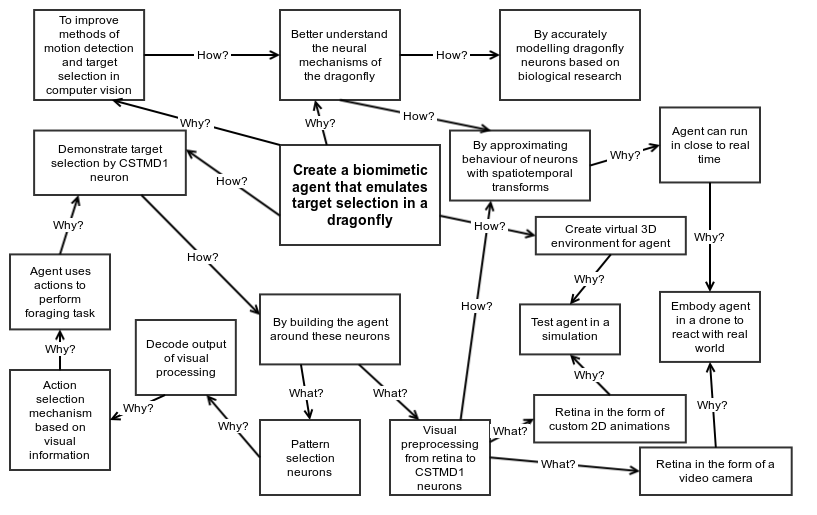
\includegraphics[scale = 0.5]{goalorient}
	\end{center}
	\caption{Goal-Oriented Capture Diagram}
	\end{figure}	
	


	
	Goal-oriented capture enabled us to establish some minimum requirements for the completion of the project. In order to build an agent that can interact with its environment and exhibit the selective function of the CSTMD1 neuron, some main objectives were originally set. Although steady progress and promising results were observed for most parts, some unexpected implications (discussed later) led to the slight modification of one of the initial goals but also to the addition of some extra goals that would significantly contribute to the overall success of the project.
\subsection{Final Specifications}
The following table summarises the finalised requirements and the level of completion for each part.
\begin{center}
    \begin{tabular}{p{12cm} c c}
    \textbf{Minimum Requirements (Stage 1)} & \textbf{Completion} \\ \hline
    (Ai) Create an animation tool to generate inputs for visual processing. & Full \\ 
	(Aii) Build a model for the ESTMD neuron present between the retina and the actual CSTMD1 neurons of a real dragonfly. & Full \\
	(Aiii) Design connection between ESTMD and CSTMD1 neurons. & Full \\
	(B) Build a layer of pattern recognition neurons that can learn to recognise spike patterns within a noisy background. & Full\\
	(C) Integrate the visual processing and pattern recognition system to detect patterns within the CSTMD1 output and add a simple action selection mechanism. & Full\\
    \end{tabular}
\end{center}

\begin{center}
    \begin{tabular}{p{12cm} c c}
    \textbf{Expected Implementation (Stage 2)} & \textbf{Completion} \\ \hline
	(A) Develop a web client to analyse metrics of each component in our model. & Full \\
	(B) Create an animation for the dragonfly agent. & Full\\
	(C) Enhance the action selection mechanism to control the agent within the environment. & Full\\
    \end{tabular}
\end{center}

\begin{center}
    \begin{tabular}{p{12cm} c c}
    \textbf{Possible Extensions (Stage 3)} & \textbf{Completion} \\ \hline
	(A) Improve the usability and features of the web client. & Full\\
	(B) Achieve CSTMD1 target selection through experimentation with various parameters and connections with the ESTMD neurons. & Partial\\
	(C) Implement the agent in a quadcopter drone. & None\\
    \end{tabular}
\end{center}




\subsection{Challenges and Motivation for Updated Specifications}
In this section, there is a brief discussion of the challenges that were faced during the project and how they motivated the adjustment of the original specifications.\par
	At the start of the project, our main objective was to create a working dragonfly target selection system. In the beginning, third party code was provided to assist with the modelling of the target selection mechanism of the CSTMD neuron. Unfortunately, although that method had been tested under specific conditions and proved successful in the past, it did not respond as expected to the visual input that was mandatory for this project. It was expected that the CSTMD neuron, when presented with two targets in the visual receptive field, would select one of them but instead of selecting one of the two targets and fire according to its movement, it merely got overstimulated firing according to the movement of both targets in the visual field. Despite the hard work that was put into addressing the issue, the complex morphology of the CSTMD neuron made the task infeasible to be fully completed within the time frame of this project. Thus, it was moved to possible extensions and although significant progress was observed, it was only partially completed by the submission deadline.\par
	What is more, to enhance the functionality of the end product as well as to enable any interested party to access and use the end product as a simulation tool, a web client was deemed a good addition to this product. The aim is for the web client to provide an interface that allows independent use of the modules as well as the connection and cooperation of the individual components for a full simulation to be ran. Key metrics are also output to demonstrate the functionality of each module and of the dragonfly visual system as a whole. 






\end{document}

